\section{Results}

\subsection{H-E1: Accommodation Patterns Are Detectable}

\begin{table}[h]
\centering
\begin{tabular}{@{}lll@{}}
\toprule
Metric & Target & Actual \\
\midrule
BCS SD & $> 0.15$ & \textbf{0.569} \\
Sample Size & $> 10,000$ & \textbf{26,395} \\
\bottomrule
\end{tabular}
\caption{H-E1 validation results.}
\label{tab:he1}
\end{table}

The BCS distribution shows substantial variance (3.8$\times$ target), confirming that accommodation is measurable.

\subsection{H-M2: AI Adapts to Human Formality}

\begin{table}[h]
\centering
\begin{tabular}{@{}lll@{}}
\toprule
Metric & Target & Actual \\
\midrule
Pearson $r$ & $> 0.1$ & \textbf{0.152} \\
$p$-value & $< 0.001$ & \textbf{$< 0.001$} \\
$n$ & Large & \textbf{111,039} \\
\bottomrule
\end{tabular}
\caption{H-M2 validation results.}
\label{tab:hm2}
\end{table}

AI response formality significantly correlates with human input formality, demonstrating accommodation behavior.

\subsection{H-M1: Users Show Weak Adaptation to AI}

\begin{table}[h]
\centering
\begin{tabular}{@{}ll@{}}
\toprule
Metric & Actual \\
\midrule
Lag-1 $r$ & \textbf{0.0134} \\
$p$-value & \textbf{0.00113} \\
\bottomrule
\end{tabular}
\caption{H-M1 validation results.}
\label{tab:hm1}
\end{table}

User adaptation is 11$\times$ weaker than AI accommodation ($r=0.013$ vs $r=0.152$).

\subsection{H-M3: Moderate Accommodation Predicts Highest Engagement}

\begin{table}[h]
\centering
\begin{tabular}{@{}lll@{}}
\toprule
Tercile & Accommodation Level & Continuation Rate \\
\midrule
T1 & High (low delta) & \textbf{65.9\%} \\
T2 & Moderate (mid delta) & \textbf{71.4\%} \\
T3 & Low (high delta) & \textbf{60.9\%} \\
\bottomrule
\end{tabular}
\caption{Continuation rates by accommodation tercile.}
\label{tab:tercile}
\end{table}

\textbf{Key finding}: T2 (moderate accommodation) shows highest continuation, not T1 (maximal accommodation). The inverted-U pattern contradicts linear CAT predictions.

\begin{figure}[h]
\centering
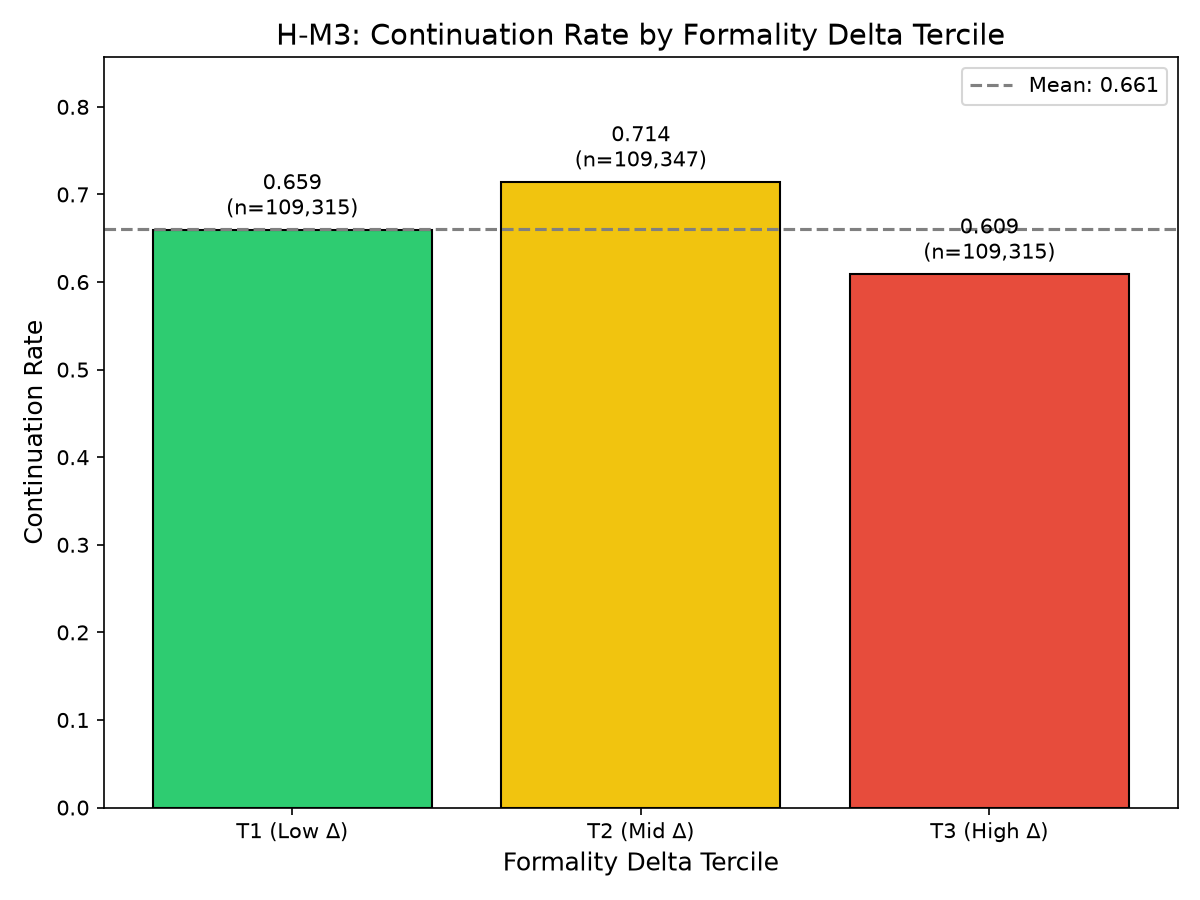
\includegraphics[width=0.8\columnwidth]{figures/tercile_bar_chart.png}
\caption{Tercile continuation rates showing inverted-U pattern.}
\label{fig:tercile}
\end{figure}
